Existing LLM serving systems were designed for single-model inference and address multi-agent workloads only partially. We identify three such challenges (\S\ref{sec:infra_challenges}), analyze application-aware systems that exploit them (\S\ref{sec:infra_scalesim}), and survey the broader landscape (\S\ref{sec:infra_landscape}).

\subsection{Multi-Agent Serving Challenges}\label{sec:infra_challenges}

Single-model serving systems (vLLM~\citep{kwon2023}, SGLang~\citep{sglang2024}, DistServe~\citep{distserve2024}) serve each request largely independently, though peer-reviewed work has begun to expose application structure: Parrot~\citep{parrot2024} passes an application-level dependency graph (semantic variables) to the scheduler, Preble~\citep{preble2025} optimizes distributed prompt sharing, Sarathi-Serve~\citep{sarathi2024} introduces chunked prefill, InferCept~\citep{infercept2024} retains KV state across tool-call interruptions, and S-LoRA~\citep{slora2024} and dLoRA~\citep{dlora2024} serve many concurrent adapters. These systems approach multi-agent serving from the general side; we return to how they differ from agent-native designs in \S\ref{sec:tension}. A recent KV cache management survey~\citep{kvcachesurvey2026} confirms that multi-agent workloads violate the per-request assumption in three ways.

\textbf{Sparse activation.} Only a fraction of agents invoke the LLM at any moment: a 1,000-agent simulation may have fewer than 10 actively generating tokens~\citep{zhou2026}. GPU memory allocated to inactive agents is wasted under conventional policies.

\textbf{Invocation distance.} Many workloads have predictable activation patterns such as sequential queues, event-driven messaging, and dependency graphs. The temporal gap before an agent's next call, termed \emph{invocation distance}~\citep{zhou2026}, is estimable from application semantics but invisible to general-purpose schedulers.

\textbf{Inter-agent memory sharing.} Agents share context (system prompts, environment descriptions, tool schemas), and general serving systems already reuse such prefixes once they appear: SGLang's RadixAttention and vLLM's automatic prefix caching both do this. What they cannot do is anticipate the \emph{application layer's} future call structure (dependency graph, message queue, execution order), so they can neither prefetch predictively nor evict semantically. This is the gap multi-agent systems target through predictive prefix management: TokenDance~\citep{tokendance2026} proposes collective KV-cache sharing across agents, DroidSpeak~\citep{droidspeak2024} enables cache reuse across different model variants, KVFlow~\citep{kvflow2025} exploits an agent step graph to evict workflow-aware and prefetch ahead of the predicted next call, and KVCOMM~\citep{kvcomm2025} aligns cache offsets across divergent per-agent prefixes so that cross-agent reuse survives the prefix change (all abstract-verified). Persistent agent-memory systems (for example A-MEM and the Mesh Memory Protocol) address a related but distinct problem, long-term memory representation rather than serving-time cache reuse, and are outside our scope.

\subsection{Application-Aware Serving}\label{sec:infra_scalesim}

Recent systems demonstrate that exploiting multi-agent workload structure yields substantial gains across four optimization axes: memory optimization, prefix-aware scheduling, cache lifecycle, and power management.

\paragraph*{Memory optimization via invocation distance.}
ScaleSim~\citep{zhou2026} introduces invocation distance as a first-class scheduling primitive. Two mechanisms exploit predictions: \emph{proactive prefetching} loads agent states before they are needed, and \emph{distance-aware eviction} replaces LRU with future-need predictions, achieving up to 1.74$\times$ speedup over SGLang~\citep{zhou2026}. Its limitation is predictable simulation workloads; interactive agents are less structured.

\paragraph*{Prefix-aware scheduling.}
TokenCake~\citep{tokencake2025} and TOPAS~\citep{topas2026} exploit shared prefixes across agents. TokenCake reports 47\% latency reduction and 16.9\% memory improvement over vLLM (abstract-verified). These figures are reported as stated by the source and are not comparable to ScaleSim's verified up to 1.74$\times$, since the two measure different quantities on different workloads. ForkKV~\citep{forkkv2026} introduces copy-on-write semantics for disaggregated KV caches, which allows efficient prefix sharing without redundant copies (abstract-verified). Prediction-based KV-cache management~\citep{predkvcache2026} applies learned policies to anticipate cache needs (abstract-verified).

\paragraph*{Cache lifecycle and power management.}
Continuum~\citep{continuum2025} introduces KV cache TTL policies for interactive tool-calling agents with unpredictable pauses (abstract-verified). KAIROS~\citep{kairos2026} introduces context-aware power management adapting GPU power states to agentic workload phases (abstract-verified). Together with ScaleSim and TokenCake, these systems illustrate that multi-agent serving requires optimization along multiple axes, and that no single system addresses the full stack.


\subsection{System Landscape}\label{sec:infra_landscape}

Table~\ref{tab:infrastructure} summarizes the broader infrastructure landscape. Beyond the application-aware systems above, infrastructure-aware orchestration (INFRAMIND~\citep{inframind2026}) bridges scheduling and placement decisions (abstract-verified). Autellix~\citep{autellix2025} provides a dedicated serving engine for LLM agents (abstract-verified), and policy-driven runtime layers~\citep{policyruntime2026} and persistent agent memory~\citep{agentmemory2026} address the system-level integration gap. Baseline serving (vLLM~\citep{kwon2023}, SGLang~\citep{sglang2024}, FlexGen~\citep{flexgen2023}) and disaggregated approaches (DistServe~\citep{distserve2024}) provide the foundation, and Mooncake~\citep{mooncake2025} extends disaggregation to a cluster-wide KV-cache pool, reporting large capacity gains under SLO on production Kimi traffic (abstract-verified). An IEEE survey~\citep{latencysurvey2026} proposes a four-layer latency optimization taxonomy, and the model-native computing architecture~\citep{modelnative2026} reconsiders the full system stack for foundation model workloads (both abstract-verified).

These systems address the four optimization axes in isolation (Figure~\ref{fig:infra_axes}). No existing system jointly optimizes all four, and none integrates diagnostic signals (\S\ref{sec:diagnostics}) into serving decisions, a gap we revisit in \S\ref{sec:discussion}.

\begin{table*}[t]
\centering
\caption{Multi-agent infrastructure systems. [a] = abstract-verified. \textbf{Pub.}: $\checkmark$ = peer-reviewed venue, $\circ$ = preprint / no confirmed venue, --- = no publication (platform/docs). Pub.\ records the venue only and is not a quality judgement.}
\label{tab:infrastructure}
\footnotesize
\setlength{\tabcolsep}{5pt}
\begin{tabular}{@{}llcc@{}}
\toprule
\textbf{System} & \textbf{Category} & \textbf{Tier} & \textbf{Pub.} \\
\midrule
ScaleSim & Memory mgmt. & 1 & $\circ$ \\
TokenCake & KV-cache sched. & 2 & $\circ$ \\
TOPAS & Prefix-aware & 2 & $\circ$ \\
KVFlow & Prefix KV-cache & 2 & $\circ$ \\
ForkKV & Copy-on-write KV & 2 & $\circ$ \\
Continuum & Cache lifecycle & 2 & $\circ$ \\
KAIROS & Power mgmt. & 2 & $\circ$ \\
TokenDance & KV sharing & 2 & $\circ$ \\
DroidSpeak & Cross-LLM KV & 2 & $\circ$ \\
Autellix & Agent serving & 2 & $\circ$ \\
INFRAMIND & Infra-aware & 2 & $\circ$ \\
KVCOMM & Cross-agent KV & 2 & $\checkmark$ \\
Mooncake & KV-cache pool & 2 & $\checkmark$ \\
Parrot & App-level DAG & 2 & $\checkmark$ \\
InferCept & KV intercept & 2 & $\checkmark$ \\
Sarathi-Serve & Chunked prefill & 2 & $\checkmark$ \\
Preble & Prompt sharing & 2 & $\checkmark$ \\
S-LoRA & Multi-adapter & 2 & $\checkmark$ \\
dLoRA & Adapter orch. & 2 & $\checkmark$ \\
vLLM & Baseline serving & 2 & $\checkmark$ \\
SGLang & Baseline serving & 2 & $\checkmark$ \\
\bottomrule
\end{tabular}
\end{table*}

\begin{figure*}[t]
\centering
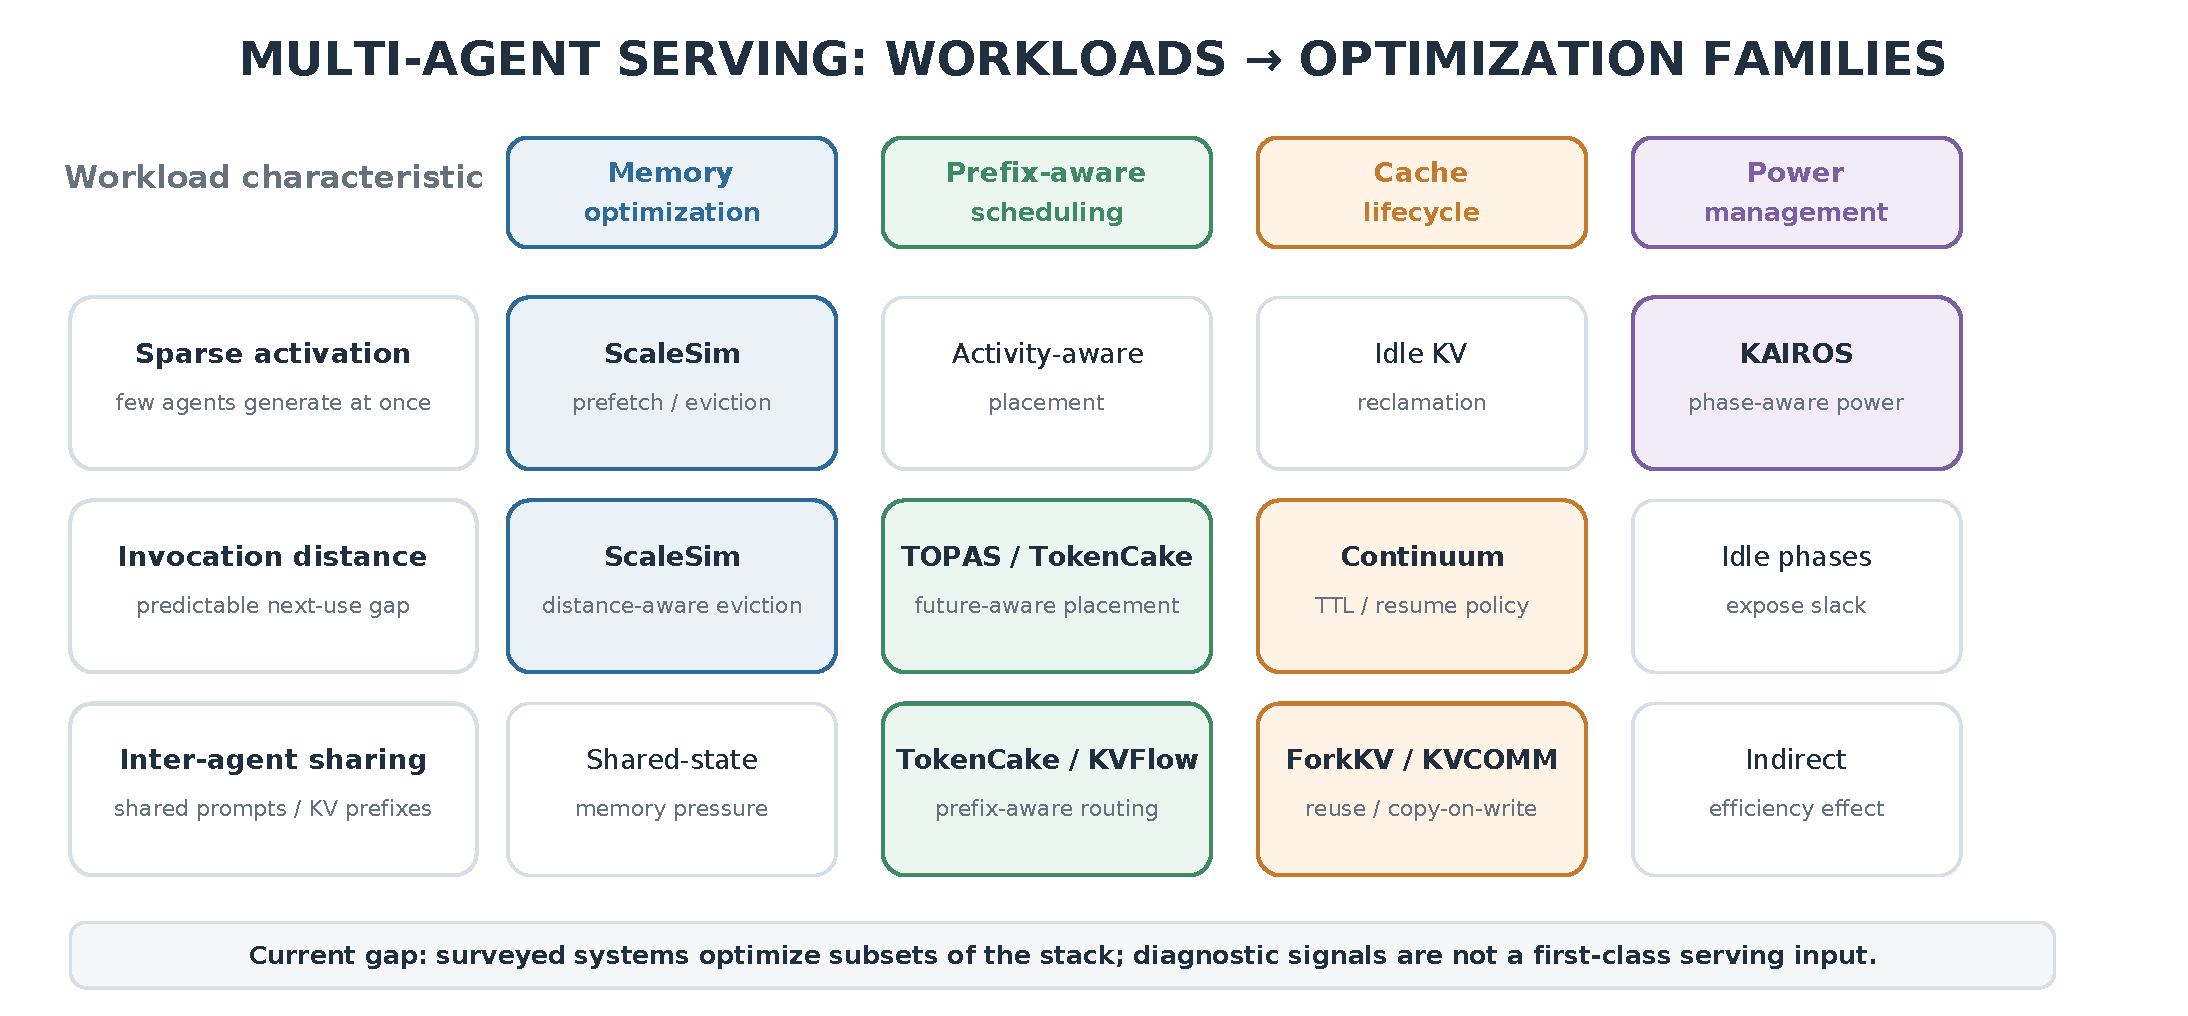
\includegraphics[width=\textwidth]{fig4_infrastructure.pdf}
\caption{Multi-agent serving challenges and optimization axes. Three workload characteristics (sparse activation, invocation distance, and inter-agent memory sharing, shown as shared prefixes in the figure) are exploited predictively by four families of application-aware systems spanning memory optimization, prefix-aware scheduling, cache lifecycle, and power management. No existing system jointly optimizes all four axes.}
\label{fig:infra_axes}
\end{figure*}